\documentclass{article}[12pt]
% \usepackage{fontspec}
% \usepackage[spanish,es-tabla, es-ucroman]{babel}

\usepackage{calc}
\usepackage{float}
\usepackage{caption}
\usepackage{graphicx}
\usepackage{pgfplotstable} 
\usepackage{enumerate} 
\usepackage{graphicx}
\graphicspath{{figuras/}}
\usepackage{parskip}
\usepackage{fancyhdr}
\usepackage{xcolor}

\usepackage[hidelinks]{hyperref}

\usepackage{lipsum}
\usepackage{setspace}


\usepackage[a4paper, total={6in, 8in},textheight=240mm]{geometry}

\usepackage{titlesec}
\usepackage{tocloft}

\usepackage{indentfirst}
\usepackage{helvet}
\renewcommand{\rmdefault}{phv}


% CONFIGURACIÓN DE LA HOJA
% \setmarginsrb{4 cm}{2.5 cm}{2 cm}{2.5 cm}{1 cm}{1.5 cm}{1 cm}{0.5 cm}

% CONFIGURACIÓN DE SANGRÍA
% \setlength{\parindent}{4mm}
% \setlength{\parskip}{1mm}

\onehalfspacing % Espaciado de 1.5 líneas

%---------------------------------------------------------------------------
%	EN TODAS HOJAS
%---------------------------------------------------------------------------

\title{Alicop}				    	% Titulo
\author{Diseño e Implementación de Arquitectura Empresarial}	            % Nombre del estudiante				
\date{\today}						        % Fecha


\makeatletter
\let\thetitle\@title
\let\theauthor\@author
\let\thedate\@date
\makeatother

\pagestyle{fancy}
\lhead{
    \begin{tikzpicture}[overlay, fill]
        \fill[ColorFondoPrimario](-4,0) rectangle(8.5,1.5);    
        \fill[ColorFondoSecundario](9,0) rectangle(10,1.5);    
    \end{tikzpicture} 
}
\rhead{
    \begin{tikzpicture}[overlay, fill]
        \node[] at (-0.2, 0.4) 
    {
\includegraphics[width=0.8cm,height=1cm]{marca_agua.png}};
    \end{tikzpicture} 
}

\rfoot{
    \begin{tikzpicture}[overlay, fill]
        \fill[ColorFondoSecundario](-20,-0.5) rectangle(5,-2.5);    
    \end{tikzpicture} 
}
\cfoot{\thepage}

\begin{document}



\titleformat{\section}
  {\normalfont\fontsize{12}{14}\bfseries} % Tamaño de la fuente (12pt) y espacio entre líneas (14pt)
  {\thesection} % Etiqueta
  {1em} % Espacio entre la etiqueta y el título
  {} % Texto adicional antes del título (vacío)


% Configuración para numerar hasta \subparagraph
\setcounter{secnumdepth}{5}
\setcounter{tocdepth}{5}
\titleformat{\paragraph}
{\normalfont\normalsize\bfseries}{\theparagraph}{1em}{}



%%%%%%%%%%%%%%%%%%%%%%%%%%%%%%%%%%%%%%%%%%%%%%%%%%%%%%%%%%%%%%%%%%%%%%%%%%%%%%%%%
%	                                CARÁTULA 
%%%%%%%%%%%%%%%%%%%%%%%%%%%%%%%%%%%%%%%%%%%%%%%%%%%%%%%%%%%%%%%%%%%%%%%%%%%%%%%%%

\pgfplotsset{compat=1.16}
% CARÁTULA
\definecolor{ColorPrimario}{RGB}{233  103  103}
\definecolor{ColorSecundario}{RGB}{120 185 40}
\definecolor{ColorFondoPrimario}{RGB}{233  103  103}
\definecolor{ColorFondoSecundario}{RGB}{145  214  92}
\begin{titlepage}
  \thispagestyle{empty}
  \newgeometry{left=2cm, right=1cm, top=2cm, bottom=2cm}

  \begin{tikzpicture}[overlay,fill]
    \fill[ColorFondoPrimario](-5,10) rectangle(20,-35);    
  \end{tikzpicture}
  
  \begin{tikzpicture}[remember picture,overlay]
    % draw image
    \node[draw] at (11.5, -10) 
    {
\includegraphics[width=16cm,height=22cm]{./figuras/background_alicorp.jpg}};
  \end{tikzpicture}
  
  \begin{tikzpicture}[overlay, fill,opacity=0.95]
    \fill[ColorFondoPrimario](-2.5,-28) rectangle(8.5,5);    
    \fill[white](-2.5, 1.5) rectangle(20,2);    
    \fill[white](-2.5,-17.5) rectangle(20,-18);    
    \fill[ColorFondoSecundario](-2.5,-28) rectangle(20,-18);    
  \end{tikzpicture}  


  \vspace{3 cm}

  \begin{minipage}{11cm}   

    \begin{flushleft}                               %alineado a ezquierda
    
    \Large \bfseries \textcolor{white}{DISEÑO E\\[0.1 cm] IMPLEMENTACIÓN DE LA }\\
    \Huge \bfseries \textcolor{white}{ARQUITECTURA EMPRESARIAL}\\
    
    \end{flushleft}

  \end{minipage}
  \vspace{\fill}

  %NOMBRE DE AUTOR
  \begin{minipage}{13cm}
    
    \begin{spacing}{1}
      \LARGE
      \begin{itemize}
        \item {Amaut Guzmán, Marcelo Fabian }
        \item {Baldeon Peña, Juancarlos }
        \item {Hernandez Ormeño, Roberth Alessandre }
        \item {Livise Larico, Rafael Enrique }
      \end{itemize}
    \end{spacing}
  \end{minipage}
  \begin{minipage}{4.5cm}
    \LARGE
    \begin{spacing}{1}
      \vspace{0.8cm}
      {U21230026}\\
      {U21201859}\\
      {1625004}\\
      {U17305723}\\
    \end{spacing}
  \end{minipage}

\end{titlepage}

%%%%%%%%%%%%%%%%%%%%%%%%%%%%%%%%%%%%%%%%%%%%%%%%%%%%%%%%%%%%%%%%%%%%%%%%%%%%%%%%%
%	                     INICIO DEL DOCUMENTO  
%%%%%%%%%%%%%%%%%%%%%%%%%%%%%%%%%%%%%%%%%%%%%%%%%%%%%%%%%%%%%%%%%%%%%%%%%%%%%%%%%



%%%%%%% ÍNDICE GENERAL
\tableofcontents
% \thispagestyle{empty} % quita numero de la pagina

%%%%%%% INDICE DE FIGURAS
\newpage
\listoffigures
% \thispagestyle{empty} % quita numero de la pagina

\newpage
% \pagenumbering{arabic} % cera numero de la pagina

%%%%%%%%%%%%%% 
% SECCIÓN 1
%%%%%%%%%%%%%%
\section{Informcion de la empresa}

\subsection{Nombre de la empresa y logo}
ALICORP SAA\\
\begin{figure}[!ht]
    \centering
    
\includegraphics[scale = 0.6]{./figuras/logo_alicorp.png}	 
    \caption{Logo de Alicorp S.A.A}
\label{fig:logo}
\end{figure}


\subsection{Rubro o giro del negocio}

\subsection{Mision}
Transformamos mercados a través de nuestras marcas líderes, generando experiencias extraordinarias en nuestros consumidores. Buscamos innovar constantemente para generar valor y bienestar en la sociedad.

\subsection{Vision}
Ser líderes en los mercados en los que competimos.
\subsection{Productos o servicios}
La sociedad tiene por objeto social dedicarse a la industria, exportación, importación, distribución y comercialización de productos de consumo masivo

\begin{itemize}
\item Consumo masivo: Alimentos, cuidado del hogar y cuidado personal
\\Aceites y Grasas: Primor, Cocinero. 
\\Harinas y Pastas: Don Vittorio, Lavaggi. 
\\Productos de Cuidado del Hogar: Bolivar, Opal. 
\\Cuidado Personal: Plusbelle, Nutribelle, etc. 
\\Alimentos y Bebidas: Aunt Jemima, Fruttis, etc. 
\\Snacks y Dulces: Chizitos, Negrita, etc. 

\begin{figure}[!ht]
    \centering
    
\includegraphics[width=0.8\textwidth]{./figuras/productos_marcas.jpg}
    \caption{Marca de algunos productos de Alicop}
    \label{fig:Marcas}
\end{figure}


\item Alicorp Soluciones: Ingredientes e insumos para los sectores de Panificación, Gastronomía y Grandes Industrias\\

\begin{figure}[!ht]
    \centering
    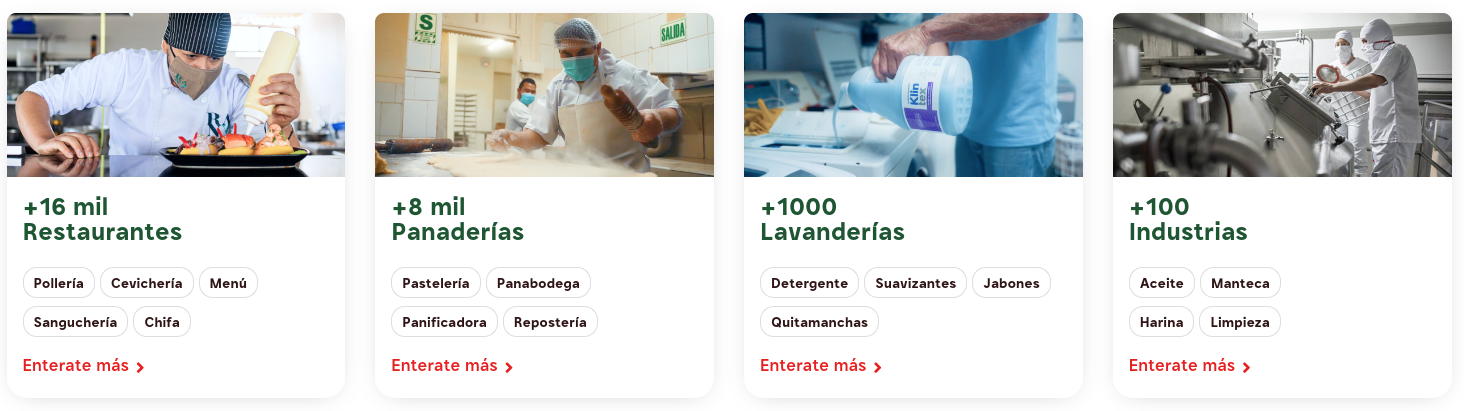
\includegraphics[width=0.8\textwidth]{./figuras/productos_alicorp_soluciones.png}
    \caption{Captura de la pagian web Alicop soluciones}
    \label{fig:alicorp_soluciones}
\end{figure}

\begin{figure}[!ht]
    \centering
    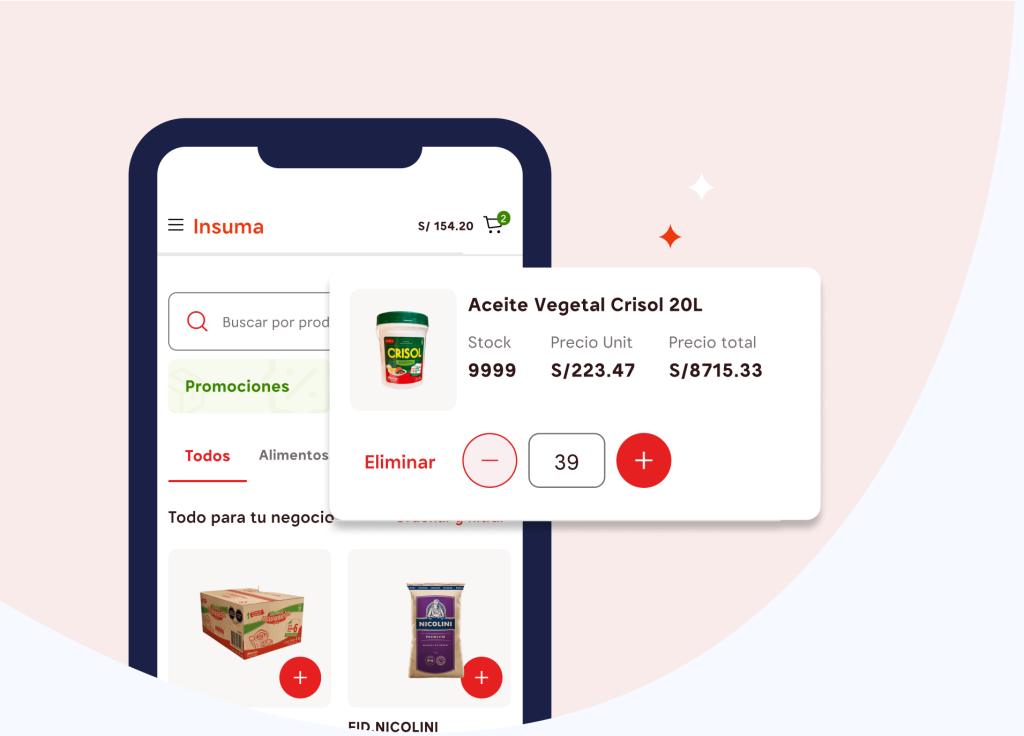
\includegraphics[width=0.8\textwidth]{./figuras/producto_insuma_app.png}
    \caption{App insuma para la logistica entre clientes}
\end{figure}

\item Acuicultura: Alimentos balanceados para camarón, salmón y peces. \\
Desde hace más de 30 años, Vitapro desarrolla soluciones especializadas en nutrición acuícola a través de sus marcas Nicovita y Salmofood, cumpliendo con los más altos estándares de calidad e innovando constantemente con el propósito de transformar la acuicultura para nutrir el mañana.
\\
\begin{figure}[!ht]
    \centering
    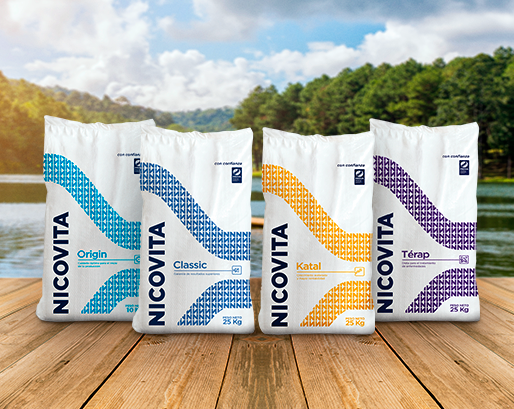
\includegraphics[width=0.6\textwidth]{./figuras/producto_nicovita.png}
    \caption{Procuto nicovita}
    \label{fig:nicovita}
\end{figure}

\end{itemize}


%%%%%%%%%%%%%% 
% SECCIÓN 2
%%%%%%%%%%%%%%

\section{Estructura Organizacional en el área de TI}

%%%%%%%%%%%%%%%%%%%%%%%%%%%%%%%%%%%%%%%%%%%%%%%%%%%%%%%%%%%%%%%%%%%%%%%%%%%%%%%%%
%	                   Políticas de TI 
%%%%%%%%%%%%%%%%%%%%%%%%%%%%%%%%%%%%%%%%%%%%%%%%%%%%%%%%%%%%%%%%%%%%%%%%%%%%%%%%%

\subsection{Políticas de TI}
\lipsum[1]
%%%%%%%%%%%%%%%%%%%%%%%%%%%%%%%%%%%%%%%%%%%%%%%%%%%%%%%%%%%%%%%%%%%%%%%%%%%%%%%%%
%	                   Objetivos de TI 
%%%%%%%%%%%%%%%%%%%%%%%%%%%%%%%%%%%%%%%%%%%%%%%%%%%%%%%%%%%%%%%%%%%%%%%%%%%%%%%%%

\subsection{Objetivos de TI}
\lipsum[1]
\subsection{Organización del área de TI}
\lipsum[1]

%%%%%%%%%%%%%%%%%%%%%%%%%%%%%%%%%%%%%%%%%%%%%%%%%%%%%%%%%%%%%%%%%%%%%%%%%%%%%%%%%
%	                   Descripción de las áreas de TI
%%%%%%%%%%%%%%%%%%%%%%%%%%%%%%%%%%%%%%%%%%%%%%%%%%%%%%%%%%%%%%%%%%%%%%%%%%%%%%%%%

\subsection{Descripción de las áreas de TI}
\subsubsection{Área de TI}
\subsubsection{Área de Infraestructura de TI}
\lipsum[1]
\subsubsection{Área de proyectos de TI}
\lipsum[1]
\subsubsection{Área de mantenimiento: }

%%%%%%%%%%%%%%%%%%%%%%%%%%%%%%%%%%%%%%%%%%%%%%%%%%%%%%%%%%%%%%%%%%%%%%%%%%%%%%%%%
%	                   CIO 
%%%%%%%%%%%%%%%%%%%%%%%%%%%%%%%%%%%%%%%%%%%%%%%%%%%%%%%%%%%%%%%%%%%%%%%%%%%%%%%%%

\subsection{CIO}
\subsubsection{Funciones}
    \begin{itemize}
        \item Gestionar el personal del área de informática. 
        \item Negociar las relaciones con los proveedores. 
        \item Supervisar la arquitectura de TI. 
        \item Definir las políticas, normas y procesos de gobernanza de las TI. 
        \item Gestionar el riesgo de la información. 
        \item Tomar decisiones sobre el gasto e inversión en TI. 
        \item Gestionar la capacidad y el ciclo de vida de la tecnología. 
        \item Comprender las tendencias tecnológicas y su aplicabilidad a los objetivos de la empresa. 
        \item Comunicar la gestión de incidentes importantes a los ejecutivos y otras partes interesadas. 
        \item Encargarse del cumplimiento de normativas gubernamentales en materia de TI 
    \end{itemize}
\subsubsection{Responsabilidades }
    \begin{itemize}
        \item Impulsar la innovación tecnológica dentro del sector en el que se desenvuelve la compañía. 
        \item Asegurar el funcionamiento continuo y el rendimiento óptimo de las plataformas y sistemas esenciales para la operación del negocio. 
        \item Trabajar de manera conjunta con los equipos de desarrollo y operaciones para garantizar la implementación puntual de soluciones tecnológicas. 
        \item Supervisar la formación y el crecimiento profesional del equipo de tecnología. 
        \item Identificar y mitigar los riesgos asociados con la seguridad de la información y los sistemas tecnológicos. 
        \item Forjar relaciones estratégicas con proveedores clave de tecnología y servicios. 
        \item Contribuir en la planificación financiera y el control de gastos en el área tecnológica. 
        \item Comunicar de forma clara y efectiva la estrategia tecnológica y los avances logrados a las partes interesadas tanto internas como externas. 
        \item Analizar cómo la tecnología influye en la productividad y eficiencia de la empresa, sugiriendo mejoras de manera constante. 
    \end{itemize}
\subsubsection{Perfil de un CIO}
El perfil de un CIO (Chief Information Officer) en una organización de gran tamaño debe reunir una sólida formación en tecnologías de la información, una visión estratégica clara y habilidades de liderazgo excepcionales. Este ejecutivo debe contar con una experiencia comprobada en la implementación de soluciones tecnológicas innovadoras que optimicen los procesos operativos y faciliten la transformación digital de la empresa. Además, es esencial que tenga la capacidad de liderar equipos multidisciplinarios, manejar proyectos tecnológicos complejos y comunicarse eficazmente con las diferentes partes involucradas. 
El CIO debe estar preparado para identificar y adoptar nuevas tecnologías de manera proactiva, que impulsen la eficiencia y competitividad de la compañía, garantizando al mismo tiempo la seguridad de la información y el cumplimiento de las normativas vigentes. También es crucial que mantenga una mentalidad estratégica que asegure la alineación de la tecnología con los objetivos corporativos, así como la creación de alianzas estratégicas con proveedores y socios clave. En resumen, el CIO ideal debe ser un líder visionario, con una sólida formación técnica y una clara orientación hacia la innovación y la eficiencia en la implementación de soluciones tecnológicas. 
\paragraph*{Especificaciones del Perfil }
    \begin{itemize}
        \item Experiencia previa en la implementación de soluciones tecnológicas en la industria de consumo masivo, debe haber liderado proyectos exitosos en la implementación de tecnología para optimizar la cadena de suministro, la producción y la distribución de productos en empresas de gran escala. Es esencial tener un historial comprobado en la mejora de procesos logísticos, automatización de plantas y sistemas de distribución. 
        \item Conocimiento profundo de las tecnologías de la información aplicadas a la producción y logística, debe estar familiarizado con tecnologías como IoT, automatización industrial, inteligencia artificial y análisis de datos, plataformas de gestión de inventario y logística, así como sistemas ERP y CRM utilizados en la industria de consumo masivo. 
        \item Habilidades de liderazgo comprobadas en entornos complejos y de alto rendimiento, debe ser capaz de liderar equipos multidisciplinarios que incluyan profesionales de TI, ingeniería, y operaciones, creando un ambiente colaborativo y orientado a resultados dentro de una industria que opera a gran escala. 
        \item Experiencia en la gestión de la seguridad de la información y protección de datos en un entorno de operaciones complejas, asegurar el cumplimiento de las normativas de seguridad de la información y la protección de datos, en especial en la privacidad del cliente y la integridad de los sistemas de producción y distribución. 
        \item Capacidad para desarrollar e implementar estrategias tecnológicas alineadas con los objetivos de crecimiento de la empresa, debe ser capaz de impulsar la innovación tecnológica que mejore la eficiencia de la producción y la distribución, optimizando procesos operativos y mejorando la agilidad en la respuesta a las demandas del mercado. 
        \item Excelentes habilidades de comunicación, es crucial que pueda colaborar eficazmente con otros líderes empresariales dentro de la organización, como las áreas de operaciones, finanzas y marketing, así como interactuar con socios estratégicos y proveedores clave en el sector de tecnología. 
        \item Experiencia en la gestión de proyectos tecnológicos complejos dentro del sector de alimentos y productos de consumo masivo: El CIO debe asegurar que los proyectos tecnológicos, como la modernización de plantas de producción o la implementación de sistemas logísticos, se entreguen a tiempo y dentro del presupuesto. 
        \item Visión estratégica para identificar oportunidades de crecimiento y optimización tecnológica: Debe poder proponer y liderar iniciativas tecnológicas que maximicen la eficiencia y el crecimiento del negocio, centrando en la sostenibilidad y la innovación en la producción y distribución de productos. 
        \item Entendimiento profundo de los desafíos del sector de consumo masivo: El CIO debe estar familiarizado con las particularidades del mercado, las tendencias de consumo y los desafíos que enfrenta una empresa de la escala de Alicorp, siendo capaz de ofrecer soluciones tecnológicas que potencien su competitividad y liderazgo en el mercado. 
    \end{itemize}
%%%%%%%%%%%%%%%%%%%%%%%%%%%%%%%%%%%%%%%%%%%%%%%%%%%%%%%%%%%%%%%%%%%%%%%%%%%%%%%%%
%	                  Diagnóstico de la Situación Actual de las TICS 
%%%%%%%%%%%%%%%%%%%%%%%%%%%%%%%%%%%%%%%%%%%%%%%%%%%%%%%%%%%%%%%%%%%%%%%%%%%%%%%%%


\subsection{Diagnóstico de la Situación Actual de las TICS}
% \subsubsection{Capacidades de las TIC’s }
% \lipsum[1]
% \subsubsection{Valoración de las capacidades de las TIC’s }
% \lipsum[1]
\subsubsection{Requerimientos del negocio}
\lipsum[1]
% \subsubsection{Requerimientos de las TIC’s}
% \lipsum[1]
% \subsubsection{Proveedores }
% \lipsum[1]



%%%%%%%%%%%%%% 
% SECCIÓN 3
%%%%%%%%%%%%%%
\section{DIAGNÓSTICO DE LA TI SITUACIÓN ACTUAL}
\subsection{Capacidades del área de TI}
    Basándonos en la información disponible, podemos inferir que Alicorp ha desarrollado un sólido ecosistema tecnológico, destacando en las siguientes áreas: 

        \paragraph*{Gestión de la Cadena de Suministro} 
        Alicorp ha invertido significativamente en la implementación de sistemas ERP (Enterprise Resource Planning) que integran y automatizan diversas funciones de la cadena de suministro, desde la planificación de la producción hasta la gestión de inventario y la distribución. Estos sistemas permiten a la empresa: 
        Optimizar la planificación de la producción: Al contar con datos precisos sobre la demanda y el inventario, Alicorp puede ajustar su producción de manera más eficiente, evitando sobrestocks y faltantes. 
        Mejorar la gestión de inventario: Los sistemas ERP permiten un seguimiento en tiempo real del inventario, lo que reduce los costos asociados a la sobreproducción o a la falta de stock. 
        Optimizar las rutas de distribución: Mediante el uso de herramientas de análisis de datos y algoritmos de optimización, Alicorp puede planificar las rutas de distribución de manera más eficiente, reduciendo costos y tiempos de entrega. 
        Aumentar la visibilidad de la cadena de suministro: El IoT (Internet de las Cosas) juega un papel fundamental al permitir el seguimiento en tiempo real de los productos a lo largo de toda la cadena de suministro, desde la materia prima hasta el consumidor final. Esto facilita la identificación de posibles problemas y la toma de decisiones más ágiles. 

        \paragraph*{Producción}
        La aplicación de las TICs en los procesos productivos de Alicorp ha permitido mejorar significativamente la eficiencia y la calidad. Algunos ejemplos son: 
        Automatización de procesos: La implementación de robots y sistemas automatizados en las líneas de producción ha reducido los errores humanos, aumentado la productividad y mejorado la seguridad de los trabajadores. 
        Control de calidad: El uso de sensores y sistemas de monitoreo en tiempo real permite detectar y corregir cualquier desviación de los estándares de calidad de manera temprana. 
        Simulación de procesos: Las herramientas de simulación permiten evaluar diferentes escenarios y optimizar los procesos productivos antes de implementarlos en la realidad, reduciendo costos y tiempo de puesta en marcha. 
    
        \paragraph*{Ventas y Marketing} 
        Alicorp ha adoptado una estrategia de marketing digital y análisis de datos para conocer mejor a sus consumidores y ofrecerles productos y servicios más personalizados. Esto se traduce en: 
        Análisis de datos: La recopilación y análisis de grandes volúmenes de datos sobre los consumidores permite identificar patrones de comportamiento, preferencias y tendencias. 
        Personalización de la experiencia del cliente: Gracias al análisis de datos, Alicorp puede ofrecer recomendaciones de productos personalizadas, campañas de marketing segmentadas y experiencias de compra más relevantes. 
        Comercio electrónico: La empresa ha desarrollado plataformas de comercio electrónico que permiten a los consumidores adquirir sus productos de manera fácil y rápida, con opciones de pago y entrega flexibles. 
        Marketing digital: Alicorp utiliza una amplia variedad de canales digitales, como redes sociales, motores de búsqueda y email marketing, para llegar a su público objetivo y generar engagement. 
    
        \paragraph*{Investigación y Desarrollo}
        Las TICs también están desempeñando un papel clave en la investigación y desarrollo de nuevos productos en Alicorp. Algunas de las aplicaciones más destacadas son: 
        Diseño asistido por computadora (CAD): El uso de software CAD permite a los ingenieros diseñar nuevos productos de manera más rápida y precisa, reduciendo los tiempos de desarrollo. 
        Simulación: Las herramientas de simulación permiten evaluar el desempeño de los nuevos productos en diferentes condiciones, lo que facilita la identificación de posibles problemas y la optimización del diseño. 
        Análisis de datos: El análisis de datos provenientes de la investigación de mercado y de los consumidores permite identificar nuevas oportunidades de negocio y desarrollar productos que satisfagan las necesidades de los consumidores. 
        
        \begin{figure}[!ht]
            \centering
            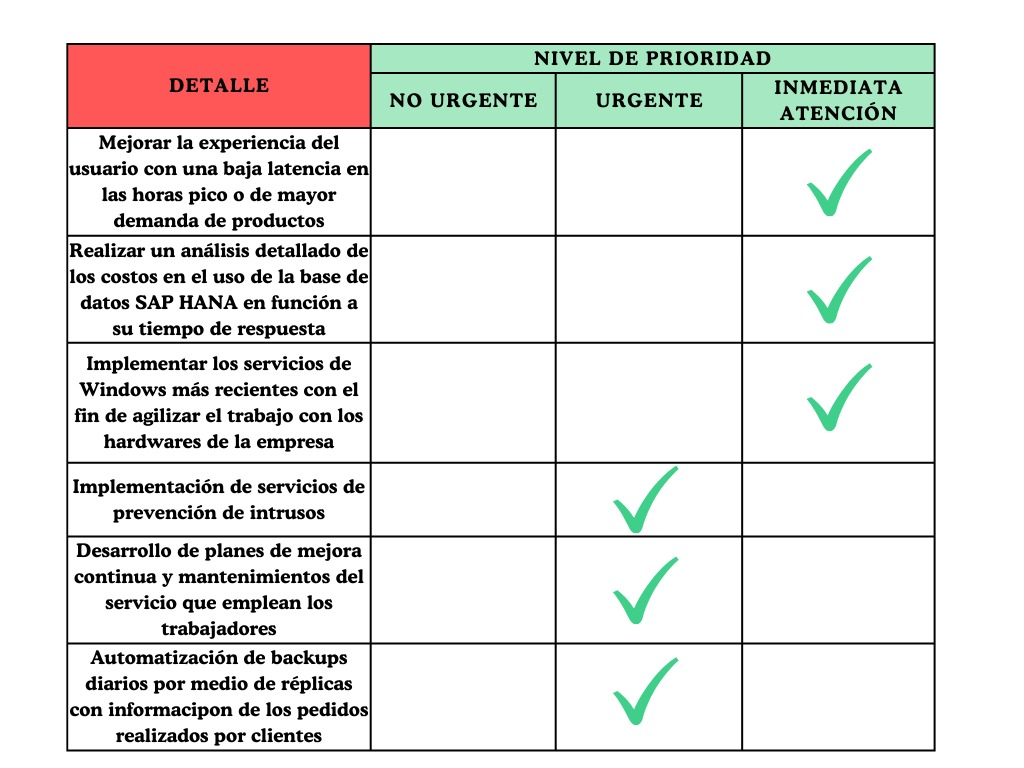
\includegraphics[width=0.9\textwidth]{backlog.jpg}
            \caption{Backlog - requerimientos del negocio}
        \end{figure}
    \newpage
    \subsubsection{Valoración de las capacidades de las TICs}
        \begin{figure}[!ht]
            \centering
            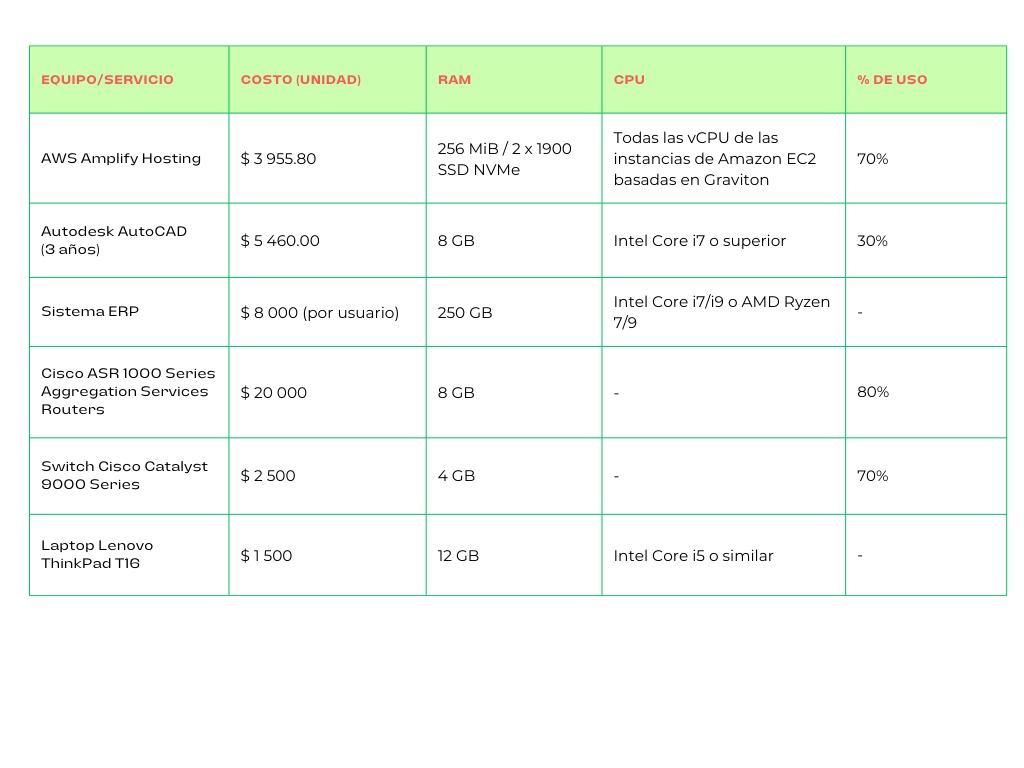
\includegraphics[width=0.8\textwidth]{cuadro_caloracion_capacidades_tic.jpeg}
            \caption{cuadro de la valoración de capacidades de las TIC's de Alicorp}
        \end{figure}

\subsection{Back log de requerimientos del negocio y del área de TI}

    \paragraph*{Automatización de Procesos Comerciales}
        \begin{itemize}
            \item Implementar un sistema que permitan a los clientes corporativos (B2B) realizar pedidos, consultar inventarios, revisar historial de compras y gestionar sus cuentas a través de una plataforma digital. Con ello, se reducirá el tiempo de procesamiento de pedidos, se minimizarán errores humanos, y se mejorará la experiencia del cliente.
            \item Implementar un software que gestione automáticamente la emisión de facturas, envíe recordatorios de pago y procese cobros, integrando todo en el sistema contable. Así se acelerará el ciclo de ventas, se mejorará en la precisión de la facturación y reducción del tiempo de respuesta en la gestión de cuentas por cobrar por el área de Logística.
            \item Desarrollar una experiencia de venta fluida y consistente, ya sea que el cliente interactúe con la marca en tiendas físicas, en línea o a través de aplicaciones móviles. Se verá mejorada la satisfacción del cliente y aumentaran las ventas al ofrecer múltiples canales de compra integrados.
        \end{itemize}
    \paragraph*{Expansión de Mercado}
        \begin{itemize}
            \item Modificar productos existentes para cumplir con las preferencias culturales, regulaciones y condiciones del mercado objetivo. Con ello se aumentarán las probabilidades de éxito al penetrar nuevos mercados ofreciendo productos que se alineen mejor con las expectativas locales.
            \item Colaborar con empresas locales o internacionales para compartir recursos y conocimientos, y entrar más eficientemente en nuevos mercados. Se reducirá el riesgo de entrada en nuevos mercados, habrá mayor acceso a la experiencia local y al capital, y gran potencial para compartir beneficios.
            \item Desarrollar campañas de marketing que se adapten a las peculiaridades de cada mercado, utilizando tanto medios digitales como tradicionales. Mejorando así la efectividad del marketing y el reconocimiento de marca en los mercados nuevos.
        \end{itemize}
    
    \paragraph*{Cumplimiento de Normativas Locales e Internacionales}
        \begin{itemize}
            \item Implementar un sistema de gestión de riesgos para asegurar el cumplimiento de las regulaciones financieras y fiscales tanto a nivel local como internacional.
            \item Realizar auditorías periódicas en la nueva sede para garantizar el cumplimiento de normativas internacionales relacionadas con la seguridad alimentaria, protección de datos y estándares laborales.
            \item Adaptar los procedimientos internos a las normativas locales, asegurando también el cumplimiento de normativas internacionales de comercio y mejores prácticas.
        \end{itemize}

    \paragraph*{Optimización de la Cadena de Suministro}
        \begin{itemize}
            \item Implementar soluciones de automatización en la logística para mejorar la eficiencia en la gestión de inventarios, reducir tiempos de entrega y asegurar el abastecimiento oportuno en la nueva operación.
            \item Integrar herramientas de análisis predictivo que permitan anticipar la demanda del mercado, optimizando el flujo de productos y materiales desde otras sedes.
            \item Fortalecer alianzas estratégicas con proveedores locales y regionales para asegurar la resiliencia de la cadena de suministro .
        \end{itemize}

\subsection{Servicios específicos brindados por proveedores y de manera interna}

\paragraph*{Google Cloud Platform (GCP)}es una plataforma de servicios en la nube que ofrece a las empresas herramientas para computación, almacenamiento, análisis de datos e inteligencia artificial, ayudando a gestionar y escalar sus operaciones tecnológicas de manera eficiente.

\paragraph*{Cisco} Cisco ofrece una amplia gama de servicios y soluciones para empresas, abarcando desde infraestructura de red y seguridad hasta colaboración y gestión de datos. 

\paragraph*{Autodesk} Autodesk ofrece software y servicios diseñados para diseñar, ingeniería y construir y crear contenido digital. Sus soluciones están orientadas a una amplia gama de industrias, incluyendo arquitectura, ingeniería, construcción, manufactura, medios y entretenimiento. 



    \subsubsection{Limitaciones y capacidades de la TI}
    \paragraph*{Capacidades:}
        Cisco proporciona soluciones avanzadas de red que permiten una conectividad segura y eficiente a nivel empresarial, mejorando la comunicación y la transferencia de datos. También ofrece herramientas de ciberseguridad robustas, como firewalls, protección contra amenazas y gestión de políticas de seguridad. Soluciones como Webex facilitan la colaboración remota y la comunicación entre equipos. Proporciona soluciones de almacenamiento y gestión de datos que facilitan la operación y administración de la infraestructura TI.
        Autodesk en un software líder para diseño 3D, CAD, ingeniería y arquitectura, facilitando la creación de modelos detallados y precisos. Sus soluciones son adaptables para diferentes sectores, incluyendo arquitectura, construcción, manufactura y medios digitales. Está constantemente innovando sus productos, integrando tecnologías como inteligencia artificial y realidad aumentada para mejorar la experiencia de usuario.
        Google Cloud crea soluciones escalables para almacenamiento, estadísticas, macrodatos y desarrollo de aplicaciones, permitiendo una adaptación a las necesidades cambiantes del negocio. Proporciona herramientas avanzadas para implementar aprendizaje automático y análisis de datos, apoyando la toma de decisiones basadas en datos. También recursos de capacitación y soporte robusto, ayudando a las empresas a adoptar sus servicios con mayor facilidad y confianza.
    \paragraph*{Limitaciones:}
        Las soluciones de Cisco suelen tener costos elevados de implementación y mantenimiento, lo que puede ser una barrera para empresas con presupuestos limitados. La implementación y gestión de las soluciones puede requerir personal altamente capacitado, aumentando la dependencia de talento especializado. Puede haber limitaciones en la integración con sistemas existentes si no se utilizan estándares compatibles.
        Los costos de licenciamiento pueden ser elevados, especialmente para empresas que requieren múltiples productos o servicios de Autodesk. La complejidad de las herramientas puede requerir una curva de aprendizaje significativa, lo cual implica inversión en capacitación para los empleados. Las aplicaciones suelen requerir hardware potente, lo que puede incrementar los costos de infraestructura TI.
        Google Cloud puede volverse impredecible debido al modelo de precios basado en uso, especialmente en empresas con un consumo elevado de recursos. Requiere una conectividad a Internet estable y rápida, lo cual puede ser un reto en zonas con infraestructura limitada. A pesar de las fuertes medidas de seguridad, algunas industrias pueden tener restricciones legales o reguladoras que dificultan el uso de servicios en la nube.
\subsection{Requerimientos del negocio}
    Desarrollar una plataforma de gestión operativa y administrativa que abarque toda la cadena de valor, desde la producción hasta la distribución, asegurando la calidad en sus productos y precios competitivos en el mercado. 
    Crear y mantener alianzas con proveedores de materias primas, distribuidores y socios tecnológicos para fortalecer la cadena de suministro y mejorar la eficiencia operativa. 
    Fomentar una relación de confianza y lealtad con los clientes a través de programas de fidelización y atención personalizada que aborden sus necesidades de manera rápida y efectiva. 
    Optimizar la logística para garantizar una distribución eficiente y oportuna de los productos en los diferentes canales de venta, minimizando tiempos de entrega y costos operativos. 
    Mantener la seguridad y el buen funcionamiento de los sistemas operativos y la infraestructura tecnológica para asegurar la continuidad del negocio y una experiencia satisfactoria para los clientes. 
    Innovar continuamente en procesos de producción y soluciones tecnológicas para mejorar la competitividad y mantener la rentabilidad del negocio. 
    Asegurar el crecimiento sostenible y la generación de valor para los accionistas mediante una gestión eficiente de los recursos y el desarrollo de productos de alto valor agregado. 
\subsection{Requerimientos de las TICs}
    Implementar soluciones tecnológicas que optimicen la gestión operativa y administrativa, garantizando la calidad y eficiencia en los procesos. 
    Mantener al personal capacitado y al tanto de nuevas tecnologías y actualizaciones en los procedimientos internos y externos. 
    Asegurar que las soluciones tecnológicas estén alineadas con los objetivos estratégicos de Alicorp y las necesidades específicas del sector de consumo masivo. 
    Evaluar e implementar tendencias tecnológicas que mejoren la competitividad de Alicorp, como la automatización en la producción, el uso de big data en la toma de decisiones y la integración de tecnologías IoT en la cadena de suministro. 
%%%%%%%%%%%%%% 
% SECCIÓN 4
%%%%%%%%%%%%%%
\section{PLANTEAMIENTO DEL PROBLEMA }
\subsection{Antecedentes del problema}

En el contexto de la expansión de Alicorp hacia Centroamérica, específicamente en El Salvador, la empresa enfrenta desafíos significativos en la optimización de su arquitectura de aplicación y TI, especialmente en el área de logística. La plataforma móvil de Insuma, que facilita la gestión de logística y ventas B2B, debe integrar eficientemente con el sistema SAP para proporcionar información actualizada sobre inventarios y pedidos. Sin embargo, la alta latencia en la comunicación entre SAP y el frontend móvil, combinada con las limitaciones en la infraestructura de red, afecta la actualización y visualización de datos críticos. Estos problemas se agravan durante los picos de demanda, impactando negativamente la eficiencia operativa y la experiencia del usuario en el área logística.

En relación con la arquitectura de aplicación de la plataforma móvil de Insuma para el área de logística de Alicorp en El Salvador, se ha implementado una solución basada en tecnologías modernas para conectar el frontend móvil con el backend que interactúa con el sistema SAP. Los módulos de SAP necesarios incluyen SAP MM (Material Management) para la gestión de inventarios, SAP SD (Sales and Distribution) para la gestión de ventas y pedidos, y SAP WM (Warehouse Management) para la administración de almacenes. La arquitectura de software del frontend móvil se basa en React Native, que permite el desarrollo de una aplicación móvil nativa con una sola base de código. El backend, construido con Node.js y Express, actúa como intermediario entre el frontend y SAP, utilizando SAP Gateway (versión 7.50) para facilitar la integración con SAP HANA como base de datos.


Para la arquitectura de datos, se ha centrado en la implementación de SAP HANA como la base de datos principal, conocida por su capacidad para manejar grandes volúmenes de datos con alta velocidad de respuesta gracias a su almacenamiento en memoria. SAP HANA permite un procesamiento de datos en tiempo real y análisis de grandes conjuntos de datos con latencias muy bajas, lo cual es crucial para las operaciones logísticas de Alicorp. Para optimizar aún más la comunicación y reducir la latencia entre el backend y SAP, se ha introducido una capa de caching con Redis. Redis, que maneja datos en memoria y ofrece tiempos de respuesta extremadamente rápidos, almacena información frecuentemente solicitada, como inventarios y precios de productos, para evitar consultas repetidas a SAP HANA. Con Redis, la capacidad de gestionar datos en caché permite una recuperación rápida de información, mientras que SAP HANA gestiona grandes volúmenes de datos con una alta eficiencia. La aplicación móvil utiliza Axios, una biblioteca de JavaScript para solicitudes HTTP, para interactuar con el backend, accediendo a los datos almacenados en Redis para respuestas rápidas o directamente desde SAP HANA cuando se necesita la información más actualizada. 

Para la arquitectura de TI, el área de logística también emplea Google Cloud Platform (GCP) para mejorar la escalabilidad y la disponibilidad de sus servicios. Utiliza Google Compute Engine para la ejecución de instancias virtuales, específicamente máquinas virtuales N2 estándar con Ubuntu 20.04 LTS como sistema operativo. Estas instancias albergan tanto el backend de Node.js como la capa de caching de Redis. Google Cloud Storage se utiliza para el almacenamiento de datos no estructurados y archivos estáticos, mientras que Google Cloud SQL ofrece una base de datos relacional adicional con MySQL 8.0 para manejar datos complementarios. La arquitectura de GCP se basa en una distribución en múltiples zonas de disponibilidad (zonas de us-central1, us-east1 y us-west1) para asegurar la alta disponibilidad y la tolerancia a fallos.

El area de logística comparte una red VPN privada basada en OpenVPN para conectar sus instalaciones logísticas en El Salvador con los servidores centrales en Sudamérica. Esta red emplea routers Cisco 2901 y tiene un ancho de banda de 20 Mbps. Aunque la latencia promedio es de 250 ms, puede aumentar durante picos de uso, afectando la sincronización de datos en tiempo real. Durante las horas pico, la red en El Salvador puede experimentar algunas interrupciones, lo que afecta la capacidad de actualizar y visualizar datos en tiempo real, incrementando moderadamente los errores en pedidos y tiempos de resolución de problemas.

En el día a día de la operación de logística en Alicorp, los usuarios de la plataforma móvil de Insuma a menudo enfrentan problemas relacionados con la alta latencia en la comunicación entre el backend y SAP. Durante los picos de demanda, como en campañas de promociones especiales o eventos de ventas, la latencia puede aumentar considerablemente, lo que resulta en tiempos de respuesta más largos al acceder a información crítica, como la disponibilidad de productos o el estado de los pedidos. Por ejemplo, si un usuario intenta consultar el inventario en tiempo real para procesar un pedido urgente y la latencia es alta, puede experimentar retrasos significativos, mostrando datos desactualizados o incorrectos sobre la disponibilidad de productos. Esto no solo afecta la eficiencia operativa, sino que también impacta negativamente en la experiencia del cliente, que puede enfrentar largos tiempos de espera o errores en sus pedidos. Además, la carga de productos en la plataforma móvil, que depende de las actualizaciones provenientes de SAP, puede verse afectada por la sincronización lenta. Esto genera problemas adicionales, como la sobrecarga en el middleware o en los servidores de caching, exacerbando la latencia y retrasando la disponibilidad de los datos en la aplicación móvil, lo cual contribuye a una experiencia de usuario frustrante y a una menor eficiencia en el procesamiento de pedidos y gestión de inventarios.

\subsection{Definición del problema}
El área de logística de Alicorp enfrenta desafíos en la gestión de inventarios y pedidos debido a limitaciones en su arquitectura de aplicaciones y en su infraestructura de TI, afectando la integración de sistemas y la sincronización de datos. Estas deficiencias impactan negativamente los pilares de aplicación y TI, comprometiendo la eficiencia operativa.

%%%%%%%%%%%%%% 
% SECCIÓN 5
%%%%%%%%%%%%%%
\input{secciones/cuerpo/seccion5.tex}

%%%%%%%%%%%%%% 
% SECCIÓN 6
%%%%%%%%%%%%%%

% %%%%%%% 1 SUBSECCIÓN %%%%%%
% \subsection{Sobre las figuras}
% Las figuras deben cumplir con los siguientes criterios: \\

% \begin{itemize}
% \item Estar numeradas y con título en la parte inferior del texto.
% \item Deben ser explicadas y citadas con su respectivo numero antes de su presentación en el documento. 
% \item Tener buena resolución. En el caso en que hayan texto, este debe estar en el idioma local.
% \item Ser citadas con su respectivo número antes de su presentación en el documento. 
% \item Las gráficas deben tener los ejes con título, unidades de medida y leyendas si necesario. El tamaño del título de los ejes y de la leyenda deben ser visibles al lector.\\
% \end{itemize} 

% La Figura \ref{fig:logo} muestra un ejemplo.

% \begin{figure}[!ht]
% \centering
% 
\includegraphics[width=0.2\textwidth]{figuras/Isotipo_NEGRO.png}
% \caption{Logo UTEC}
% \label{fig:logo}
% \end{figure}

% %%%%%%% 2 SUBSECCIÓN %%%%%%

% \subsection{Sobre las tablas}
% Sigue algunos criterios a tener en cuenta en el momento de presentar tablas:\\

% \begin{itemize}
% \item Deben estar numeradas y con título en la parte inferior del texto.
% \item Deben ser explicadas y citadas con su respectivo número antes de su presentación en el documento. 
% \item Las magnitudes de estudio deben estar identificadas (ej. datos, sitio, potencia, y otros), acompañada de su unidad de medida siempre que haya. En caso de que se utilicen símbolos, estos deben ser explicados en el texto. 
% \item Los valores  deben ser escritos teniendo en cuenta las cifras significativas que indique el docente responsable.
% \item Para números muy grandes o pequeños se debe usar notación científica.\\
% \end{itemize}

% Ejemplos:

% \begin{table}[htb]
% \begin{center}
% \renewcommand\arraystretch{1.3}
% \centering
% \begin{tabular} {c c c c}
%  \hline
% N° & t (s) & I (W/m$^{2}$) & d (m)\\
%  \hline
% 1 & 1,23 & 4200 & 1,20\\
% 2 & 1,25 & 3997 & 1,50\\
% 3 & 1,23 & 4200 & 1,20\\
%  \hline
%  \end{tabular}
%  \caption{Valores experimentales de la práctica X}
% \label{ta:tab1}
%     \end{center}
%  \end{table}
 
% \begin{table}[htb]
% \begin{center}
% \begin{tabular}{l c c}
% \hline
% Mes & $\mathrm{HSP_{PH} (h)}$ & $\mathrm{HSP_{PI} (hrs)}$ \\
% \hline
% Enero & 224 & 213\\ 
% Julio & 224 & 213\\ 
% Diciembre & 224 & 213\\ 
% \hline
% \end{tabular}
% \caption{Ejemplo 2 de tabla}
%     \end{center}
% \label{tab:ValoresHSP}
% \end{table}

% %%%%%%%%%%%%%% 
% % SECCIÓN 7
% %%%%%%%%%%%%%%
% \section{Conclusiones}
% Este sección debe cerrar la propuesta del trabajo. Algunos criterios para la redacción: \\

% \begin{itemize}
% \item Ser objetivo. 
% \item Retomar la propuesta inicial y vincular con los resultados obtenidos.
% \item Realizar un análisis critico, proponer mejoras y estudios futuros.
% \end{itemize}

% %%%%%%%%%%%%%% 
% % SECCIÓN 8
% %%%%%%%%%%%%%%
% \section{Características de la bibliografía}
% La sección bibliográfica debe estar ordenada alfabéticamente por apellido del autor. Se recomienda la utilización del formato APA (American Psychological Association).

% %%%%%%%%%%%%%% 
% % SECCIÓN 9
% %%%%%%%%%%%%%%
% \section{Características de los anexos}

% \begin{itemize}
% \item Pueden ser documentos de distinta índole, que aporten información complementaria o aclaratoria de cierto aspecto de la obra. 
% \item Si fueron extraídos de fuentes consultadas, se deberán incluir sus referencias. 
% \item Deben estar incorporados en el orden en que fueron mencionados en el desarrollo del trabajo.
% \end{itemize}


\end{document}
